\documentclass[twoside,UTF8]{EPURapport}
%\usepackage{listings}

%\renewcommand{\lstlistlistingname}{Liste des codes}
%\renewcommand{\lstlistingname}{Code}

%\addextratables{%
%	\lstlistoflistings
%}

%\swapAuthorsAndSupervisors
\nolistoffigures
\nolistoftables


\usepackage{amsmath}
\usepackage{amsfonts}
\usepackage{amssymb}

\usepackage{float}
%\usepackage{color}
\usepackage{array}
\usepackage{multirow}
%\usepackage{xcolor}
\usepackage{supertabular}
\usepackage{longtable}
\usepackage{algorithmic}
\usepackage{algorithm}
\usepackage{hyperref}

\usepackage{graphicx}
\usepackage{caption}
\usepackage{subcaption}


\renewcommand{\algorithmicrequire}{\textbf{Entrées et pr\'{e}condition:}}
\renewcommand{\algorithmicensure}{\textbf{Sorties et postcondition:}}
\renewcommand{\algorithmicend}{\textbf{fin}}
\renewcommand{\algorithmicif}{\textbf{si}}
\renewcommand{\algorithmicthen}{\textbf{alors}}
\renewcommand{\algorithmicelse}{\textbf{sinon}}
\renewcommand{\algorithmicelsif}{\algorithmicelse\ \algorithmicif} 
\renewcommand{\algorithmicendif}{\algorithmicend\ \algorithmicif} 
\renewcommand{\algorithmicfor}{\textbf{pour}}
\renewcommand{\algorithmicforall}{\textbf{pour tout}} 
\renewcommand{\algorithmicdo}{\textbf{faire}}
\renewcommand{\algorithmicendfor}{\algorithmicend\ \algorithmicfor} 
\renewcommand{\algorithmicwhile}{\textbf{tant que}}
\renewcommand{\algorithmicendwhile}{\algorithmicend\ \algorithmicwhile} 
\renewcommand{\algorithmicloop}{\textbf{boucle}}
\renewcommand{\algorithmicendloop}{\algorithmicend\ \algorithmicloop} 
\renewcommand{\algorithmicrepeat}{\textbf{répéter}}
\renewcommand{\algorithmicuntil}{\textbf{jusqu'à}}
\renewcommand{\algorithmictrue}{\textbf{vrai}}
\renewcommand{\algorithmicfalse}{\textbf{faux}}
\renewcommand{\algorithmiccomment}[1]{$/*$~#1~$*/$}
\floatname{algorithm}{Algorithme}
\renewcommand{\listalgorithmname}{Liste des algorithmes}

\thedocument{Rapport de validation}{Développement d’un outil de traitement d’images par filtrage bilatéral}{Validation de l'implémentation du filtre bilatéral}

\grade{Département Informatique\\ 5\ieme{} année\\ 2014 - 2015}

\authors{%
	\category{Étudiants}{%
		\name{Natacha \textsc{Marlio-Ma}} \mail{natacha.marlio-marette@etu.univ-tours.fr}
	}
	\details{DI5 2014 - 2015}
}

\supervisors{%
	\category{Encadrants}{%
		\name{Moncef \textsc{Hidane}} \mail{moncef.hidane@insa-cvl.fr}
	}
	\details{INSA, Blois}
}

\abstracts{}
{}
{}
{}

\begin{document}


\chapter{Implémentation du filtre bilatéral}

\paragraph{}
L'implémentation du filtre bilatéral se base sur un algorithme d'un article  \cite{filtreBilateral} voir ci-dessous \ref{algo:impFB}. Soit \textbf{p} un pixel de l'image \textbf{S} avec pour valeur \textbf{$I_{p}$}. $\|.\|$ représente une distance euclidienne et |.| représente une valeur absolue. Le résultat du filtre bilatéral de l'image noté BF[.]. $G_{\sigma}(x)$ représente une fonction gaussienne, ici de la forme : 

\begin{align}
	G_{\sigma}(x) = \frac{1}{2\pi \sigma} \exp(-\frac{x^2}{2\sigma^2})
\end{align}

\begin{algorithm}[H]
\caption{Implémentation naïve du filtre bilatéral}
\label{algo:impFB}
\algsetup{indent=3em}
\begin{algorithmic}[1]
\FOR[Parcours de chaque pixel de l'image S]{chaque pixel \textbf{p} de \textbf{S}}	
	\STATE $BF[I]_p =0$
	\COMMENT{Initialisation}
	\STATE $W_p = 0$
	\FOR[]{chaque pixel \textbf{q} de \textbf{S}}
		\STATE $w = G_{\sigma_s}(\|p-q\|)G_{\sigma_r}(|I_p-I_q|)  $
		\STATE $BF[I]_p += wI_q$
		\STATE $W_p += w$
	\ENDFOR
	\STATE $BF[I]_p = I_p / W_p$
	\COMMENT{Normalisation} 
\ENDFOR

\end{algorithmic}
\end{algorithm}

\paragraph{}
Dans l'implémentation réalisée, la deuxième boucle for ne parcours pas comme dans l'algorithme toute l'image mais seulement une fraction de celle-ci. Le parcours du pixel \textbf{q} se fait dans un cadre de 21x21 pixels autour du pixel courant \textbf{p}. Si le cadre dépasse de l'image, on considère que les valeurs des pixels devant être en dehors seront nuls. Cela ne revient à ne considérer que les pixels du cadre appartenant à l'image. 

\paragraph{}
Si l'image est en couleur au lieu d'être en niveaux de gris, le parcours de l'image se fait le nombre de fois qu'il y a de canaux, c'est à dire trois fois pour une image RGB. Le filtre bilatéral sera calculé pour chaque canal de l'image. 

\paragraph{}
Le filtre bilatéral implémenté est dépendant de deux paramètres $\sigma_s$ et $\sigma_r$. $G_{\sigma_{s}}$ est une gaussienne spatiale qui permet de diminuer l'influence des pixels distants. $G_{\sigma_{r}}$ est une gaussienne de gamme qui diminue l'influence d'un pixel \textbf{q} lorsque son intensité diffère \textbf{$I_p$}.


\chapter{Validation}

La validation du filtre bilatéral s'est faîte en deux étapes. La première consistait à vérifier que le filtre bilatéral reproduisait correctement le comportement d'un filtre gaussien, c'est à dire de convolution gaussienne. Une valeur grande de $\sigma_r$ permet d'approcher une convolution gaussienne car la valeur de $G_{\sigma_r}$ diminue et tend vers un. La convolution gaussienne ne tient compte que de la gaussienne spatiale ($G_{\sigma_s}$). 
La seconde étape permet de vérifier que les résultats obtenus concordent avec ceux de l'implémentation du filtre bilatéral de CImg. Pour cela deux pourcentages sont calculés : un premier correspondant au pourcentage maximum de différence entre les valeurs des deux images obtenues (équation \ref{diffPixel}) et un deuxième correspondant au pourcentage de différence entre les deux images (équation \ref{diffImage}).

\begin{equation}\label{diffPixel}
	diffPixel = \max_{i, y} \frac{\sum\limits_{c}\frac{I_{fb,c} - I_{CImg,c}}{255} * 100}{c} 
\end{equation}
\begin{equation}\label{diffImage}
	diffImage = \frac{\sum\limits_{x} \sum\limits_{y} \sum\limits_{c} \frac{I_{fb,c} - I_{CImg,c}}{255} * 100 }{x*y*c}
\end{equation}

\paragraph{}
La comparaison se fait avec des images initiales bruitées par un bruit gaussien. On accepte un pourcentage de différence entre l'image produite avec CImg et celle produite avec l'implémentation du filtre bilatéral de 5\% au maximum. 

\chapter{Résultats}

\paragraph{}
Les images ci-dessous ont été obtenues avec le filtre bilatéral implémenté. 

\begin{figure}[H]
	\begin{center} 
		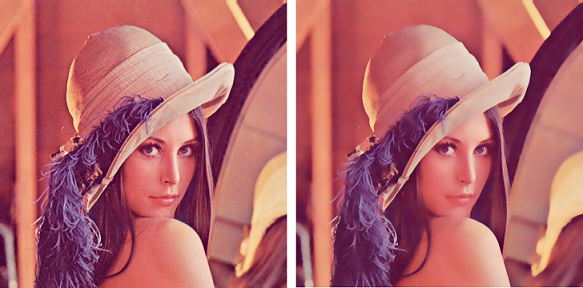
\includegraphics[scale=0.7]{images/lena_4_30.png} 
	\end{center} 
	\caption{Filtrage bilatéral avec $\sigma_s$=4 et $\sigma_r$=30 }
\end{figure} 

\begin{figure}[H]
	\begin{center} 
		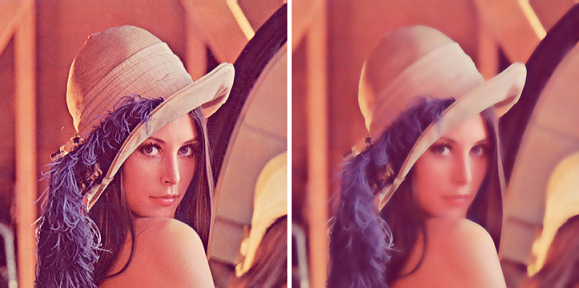
\includegraphics[scale=0.7]{images/lena_4_70.png} 
	\end{center} 
	\caption{Filtrage bilatéral avec $\sigma_s$=4 et $\sigma_r$=70 }
\end{figure} 

\begin{figure}[H]
	\begin{center} 
		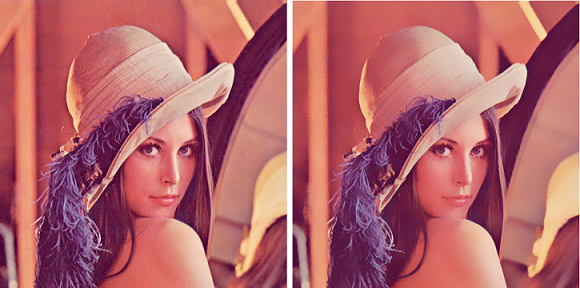
\includegraphics[scale=0.7]{images/lena_64_20.png} 
	\end{center} 
	\caption{Filtrage bilatéral avec $\sigma_s$=64 et $\sigma_r$=20 }
\end{figure} 

\begin{figure}[H]
	\begin{center} 
		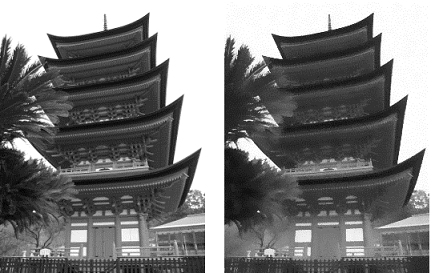
\includegraphics[]{images/IM088_4_30.png} 
	\end{center} 
	\caption{Filtrage bilatéral avec $\sigma_s$=4 et $\sigma_r$=30 }
\end{figure} 

\begin{figure}[H]
	\begin{center} 
		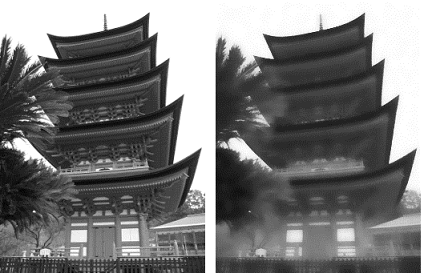
\includegraphics[]{images/IM088_4_70.png} 
	\end{center} 
	\caption{Filtrage bilatéral avec $\sigma_s$=4 et $\sigma_r$=70 }
\end{figure} 

\begin{figure}[H]
	\begin{center} 
		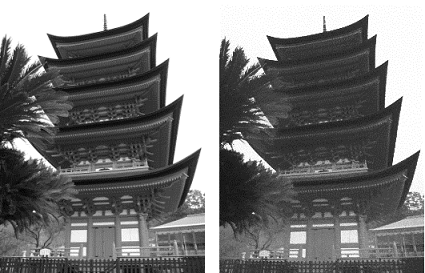
\includegraphics[]{images/IM088_64_30.png} 
	\end{center} 
	\caption{Filtrage bilatéral avec $\sigma_s$=64 et $\sigma_r$=30 }
\end{figure} 

\bibliography{biblio}
\bibliographystyle{unsrt}
\addcontentsline{toc}{chapter}{Bibliographie}

\end{document}